\chapter{Distance-Based Approach for Natural Transitions}
\label{Chapter3}

Building upon the system architecture presented in Chapter~\ref{Chapter2}, this chapter details our \textbf{distance-based} approach for creating natural transitions between fixed and procedurally generated terrain. The algorithms highlighted in this chapter are applied as \textit{post-processing} modifications to change the heights set by normal procedural terrain generation techniques to now blend into the constrained areas of the terrain. As an example, these distance-based modifiers would be applied to terrains in the state as seen in Fig. \ref{fig:top_down_example}, when we describe our top-down approach in Section \ref{top_down_approach}. We present the mathematical foundations and algorithmic innovations that enable seamless terrain integration while preserving exact height constraints. 

\textbf{Notation}: Throughout this chapter, we use $n$ to denote the total number of pixels in the terrain heightmap, where $n = w \times h$ for a terrain of width $w$ and height $h$. This notation simplifies our complexity analysis as most terrain operations process pixels rather than dimensions separately.

\subsubsection{Conceptual Foundation}

The central insight of our approach is that \textbf{distance from fixed points} provides an effective metric for controlling terrain modifications. Rather than applying uniform operations across all modifiable terrain, we modulate operation strength based on \textbf{proximity} to constraints.

This distance-based methodology emerged from observing that abrupt transitions at constraint boundaries (illustrated in Figure~\ref{fig:constraint_discontinuity}) result from treating all modifiable points equally. By introducing distance-aware processing, we create what can be conceptualised as a ``field of influence'' originating from fixed areas. The key principles are:


\begin{itemize}
    \sloppy
    \item \textbf{Proximity-based modification}: Modifications apply with varying strength based on distance to fixed points;
    \item \textbf{Detail preservation}: Areas far from constraints maintain (previously) procedurally generated characteristics;
    \item \textbf{Natural gradients}: Smooth transitions emerge from the distance-based modifications.
\end{itemize}


As we established in the earlier chapters, this approach offers several advantages over the constraint-specific methods. For example, unlike \textcite{Belhadj07}'s \textit{bottom-up} method designed for connected constraints, our approach handles \textbf{arbitrary} constraint patterns. While \textcite{Andereck14}'s path-based method excels with linear features, our methodology generalises to \textit{any} constraint configuration. 

Additionally, our approach works as a \textbf{modulation layer} compatible with any terrain generation algorithm. It is simply an additional step, independent from any specificities of implementations of the terrain generation technique.

The primary trade-off is computational simplicity versus specialisation. While dedicated approaches may produce marginally superior results for their specific constraint types, our method provides consistent quality across all constraint patterns while maintaining the efficiency needed for interactive use and parameter exploration through the Interactive Genetic Algorithm (Chapter~\ref{Chapter4}).


\subsubsection{Distance Grid Calculation}
\label{distance_grid_calculation}

The distance grid forms the foundation of our approach, storing the minimum distance from each terrain point to the nearest fixed point. This is an idea we came up with when trying to figure out how to get gentle transitions between the constrained and modifiable areas. While Chapter \ref{Chapter2} introduced this data structure conceptually, we now present its mathematical definition and efficient computation.

Let $M$ be a binary mask that defines fixed points on the terrain (i.e., $M(x, y) = \text{true}$ indicates a fixed point). We define the distance grid $D$, where each entry $D(x, y)$ represents the Euclidean distance from point $(x, y)$ to the nearest fixed point:

\[D(x, y) = \min_{(i,j) \in F} || (x,y) - (i,j) ||_2 \]
Here, $F = \{(i,j) \mid M(i,j) = \text{true}\}$ is the set of all fixed points, and $\left\| \cdot \right\|_2$ denotes the Euclidean norm. The grid $D$ is defined over the entire terrain heightmap, with one value $D(x, y)$ for each coordinate $(x, y)$.

We compute the distance grid using a \textbf{breadth-first search} algorithm that propagates distances outward from fixed points. The algorithm achieves $O(n)$ time complexity, making it practical even for large terrains.

The computed distance grid enables all subsequent distance-aware operations, serving as a shared data structure that eliminates redundant distance calculations across multiple terrain operations.

\section{Enhanced Distance-Based Smoothing}
\label{edbs}

Our enhanced distance-based smoothing algorithm creates natural transitions by applying variable smoothing strength based on proximity to fixed points. Unlike uniform smoothing that treats all points equally, our approach preserves more terrain detail further away from the fixed points, while ensuring seamless integration at constraint boundaries.

The algorithm operates on two key principles:

\begin{enumerate}
    \item \textbf{Distance-adjusted strength}: Smoothing intensity decreases with distance from fixed points;
    \item \textbf{Directional weighting}: Neighbours closer to fixed areas receive additional weight, creating a ``pull'' effect.
\end{enumerate}

This combination produces organic blending that appears as if the terrain \textit{naturally} conforms to the fixed elements, rather than exhibiting artificial smoothing artifacts.

\subsubsection{Mathematical Formulation}
\label{edbs_math}

For each modifiable point $(x, y)$, we calculate the \textbf{smoothed height} as a weighted average:

\[h'(x, y) = \frac{\sum_{(i,j) \in N(x,y)} w(i,j) \cdot h(i,j)}{\sum_{(i,j) \in N(x,y)} w(i,j)}
\]

where:

\begin{itemize}
    \item $h'(x,y)$ represents the new smoothed height at position $(x,y)$;
    \item $h(i,j)$ is the original height at position $(i,j)$;
    \item $N(x,y)$ is the set of all neighbouring points (including the centre point itself);
    \item $w(i,j)$ is the weight assigned to each neighbour.
\end{itemize}
 

\hfill


The \textbf{weight function} combines distance-based and directional effects:

\[w(i,j) = \begin{cases}
1.0 & \text{if } (i,j) = (x,y) \\
s \cdot (1 - d_{norm}(x,y)) \cdot p(i,j) & \text{otherwise}
\end{cases}
\]
where each component serves a specific purpose:
\begin{itemize}
    \item $(x,y)$ is the current point being smoothed;
    \item $s$ is the base smoothing factor controlling overall smoothing strength;
    \item \(d_{norm}(x,y) = \frac{D(x,y)}{\max_{(a,b)} D(a,b)}\)  is the normalised distance, where:
        \begin{itemize}
            \item $D(x,y)$ is the distance from point $(x,y)$ to the nearest fixed point;
            \item $\max_{(a,b)} D(a,b)$ is the maximum distance value in the entire distance grid.
        \end{itemize}
    Thus, $d_{norm} \in [0, 1]$, with 0 at fixed points and 1 at the farthest points.
    \item $1 - d_{norm}(x,y)$ creates distance-based falloff: 
        maximum effect (1.0) at fixed boundaries, minimum effect (0.0) at maximum distance;
    \item $p(i,j)$ is the directional proximity factor:
        \[p(i,j) = \begin{cases}
        c & \text{if } D(i,j) < D(x,y) \text{ (neighbour is closer to fixed points)} \\
        1.0 & \text{otherwise}
        \end{cases}\]
    
    \item $c$ is the proximity weight multiplier that amplifies the influence of neighbours closer to fixed areas.
\end{itemize}

The centre point weight of \textbf{1.0} ensures stability by preventing the smoothed value from deviating too far from the original height in a single iteration.

\subsubsection{Implementation}

For more clarity, we also include a pseudocode of the core algorithm in \ref{alg:enhanced_smoothing}:

\begin{algorithm}[H]
% \small
\caption{Enhanced Distance-Based Smoothing}
\label{alg:enhanced_smoothing}
\begin{algorithmic}[1]
\Require $\text{heightMap}[w \times h]$, $\text{distanceGrid}[w \times h]$, $\text{params}$
\Ensure Smoothed heightMap respecting distance-based constraints

\State $\text{maxDistance} \gets \max(\text{distanceGrid})$
\For{$\text{iteration} = 1$ to $\text{params.iterations}$}
    \State $\text{originalHeights} \gets \text{copy}(\text{heightMap})$
    
    \For{each modifiable point $(x,y)$}
        \State $d_{\text{norm}} \gets \text{distanceGrid}[x,y] / \text{maxDistance}$
        \State $\text{smoothingFactor} \gets \text{params.baseSmoothing} \times (1 - d_{\text{norm}})$
        
        \State $\text{weightedSum} \gets \text{originalHeights}[x,y]$ \Comment{Center weight = 1.0}
        \State $\text{totalWeight} \gets 1.0$
        
        \For{each neighbor $(n_x, n_y) \in N(x,y) \setminus \{(x,y)\}$}
            \State $\text{weight} \gets \text{smoothingFactor}$
            
            \If{$\text{distanceGrid}[n_x, n_y] < \text{distanceGrid}[x,y]$}
                \State $\text{weight} \gets \text{weight} \times \text{params.proximityWeight}$
            \EndIf
            
            \State $\text{weightedSum} \gets \text{weightedSum} + \text{originalHeights}[n_x, n_y] \times \text{weight}$
            \State $\text{totalWeight} \gets \text{totalWeight} + \text{weight}$
        \EndFor
        
        \State $\text{heightMap}[x,y] \gets \text{weightedSum} / \text{totalWeight}$
    \EndFor
\EndFor
\end{algorithmic}
\end{algorithm}

\textbf{Complexity Analysis}: The algorithm has time complexity $O(k \times n)$ where $k$ is the number of iterations and $n$ is the total number of pixels. Each iteration processes all modifiable pixels (at most $n$), and for each pixel examines exactly 8 neighbours (a constant-time operation). The practical impact of $k$ is significant: with high values of iterations (e.g., $k = 100$) , we may introduce noticeable latency. The GPU implementation achieves near-constant time per iteration through massive parallelisation, effectively reducing the complexity to $O(k)$ with sufficient parallel processing units. The actual time analysis and comparison between this algorithm in its CPU and GPU implementation will be discussed in Chapter \ref{Chapter5}.

We also include several figures to illustrate the results of our methods. For example, Figure \ref{fig:smoothing_comparison} demonstrates the advantage of our approach over uniform smoothing, and illustrates how our two-stage approach solves the boundary problem identified in Chapter~\ref{Chapter1}. Figure \ref{fig:close_up_transition} shows how the technique creates seamless transitions at constraint boundaries\footnote{The algorithm is GPU-accelerated for real-time performance, with automatic CPU fallback for compatibility.} \footnote{For parameter tuning guidelines, refer to the user documentation.}.

\begin{figure}[h]
    \centering
    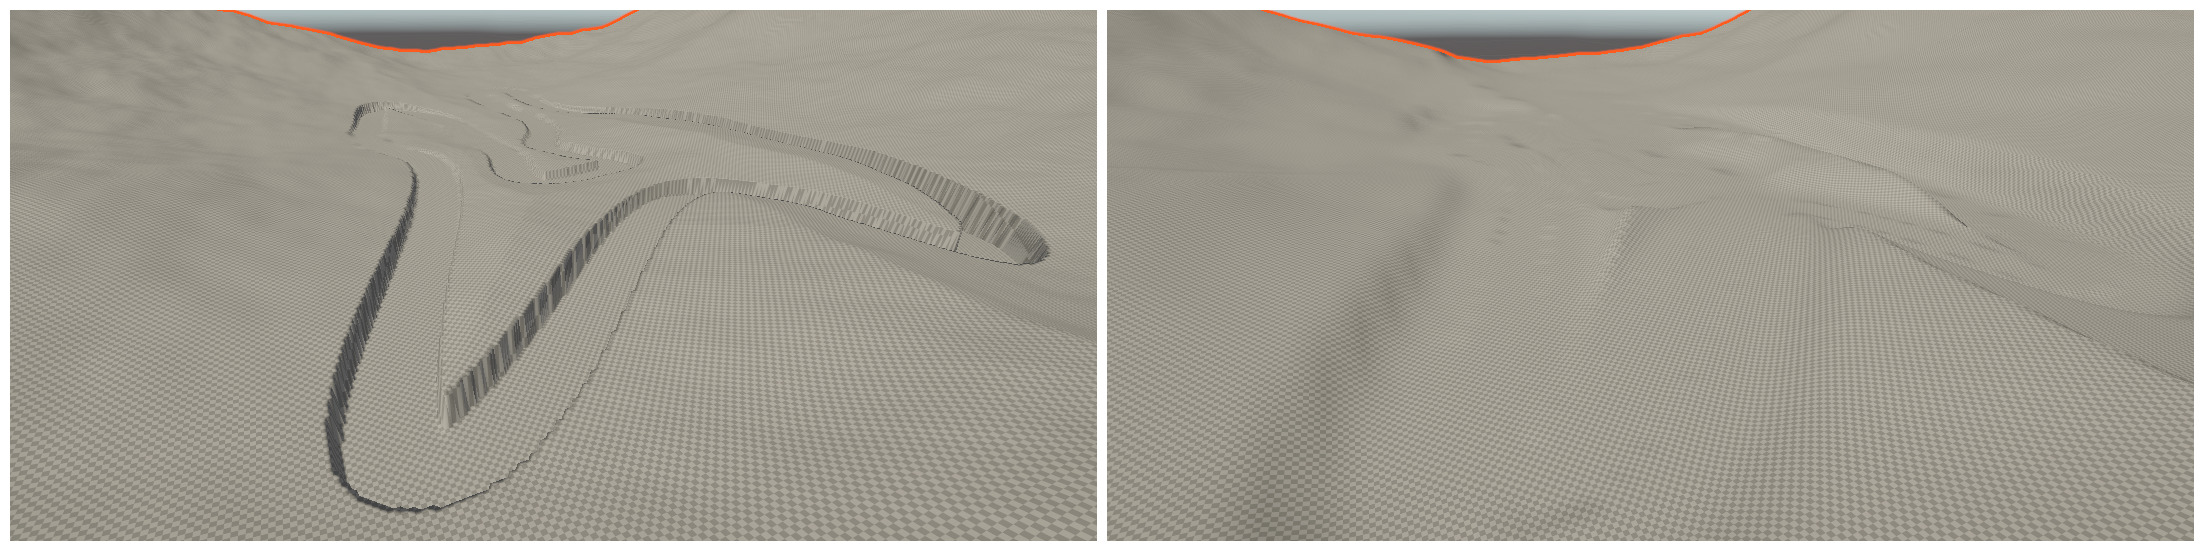
\includegraphics[width=1.0\textwidth]{img/distance_based_images/close_up_transition.jpg}
    \caption{Close-up comparison of terrain transitions. (Left) After distance-based height scaling (described in Section \ref{dbhs}), showing visible but manageable elevation differences. (Right) After enhanced distance-based smoothing, demonstrating seamless integration between fixed and generated terrain.}
    \label{fig:close_up_transition}
\end{figure}


\begin{figure}[h!]
    \centering
    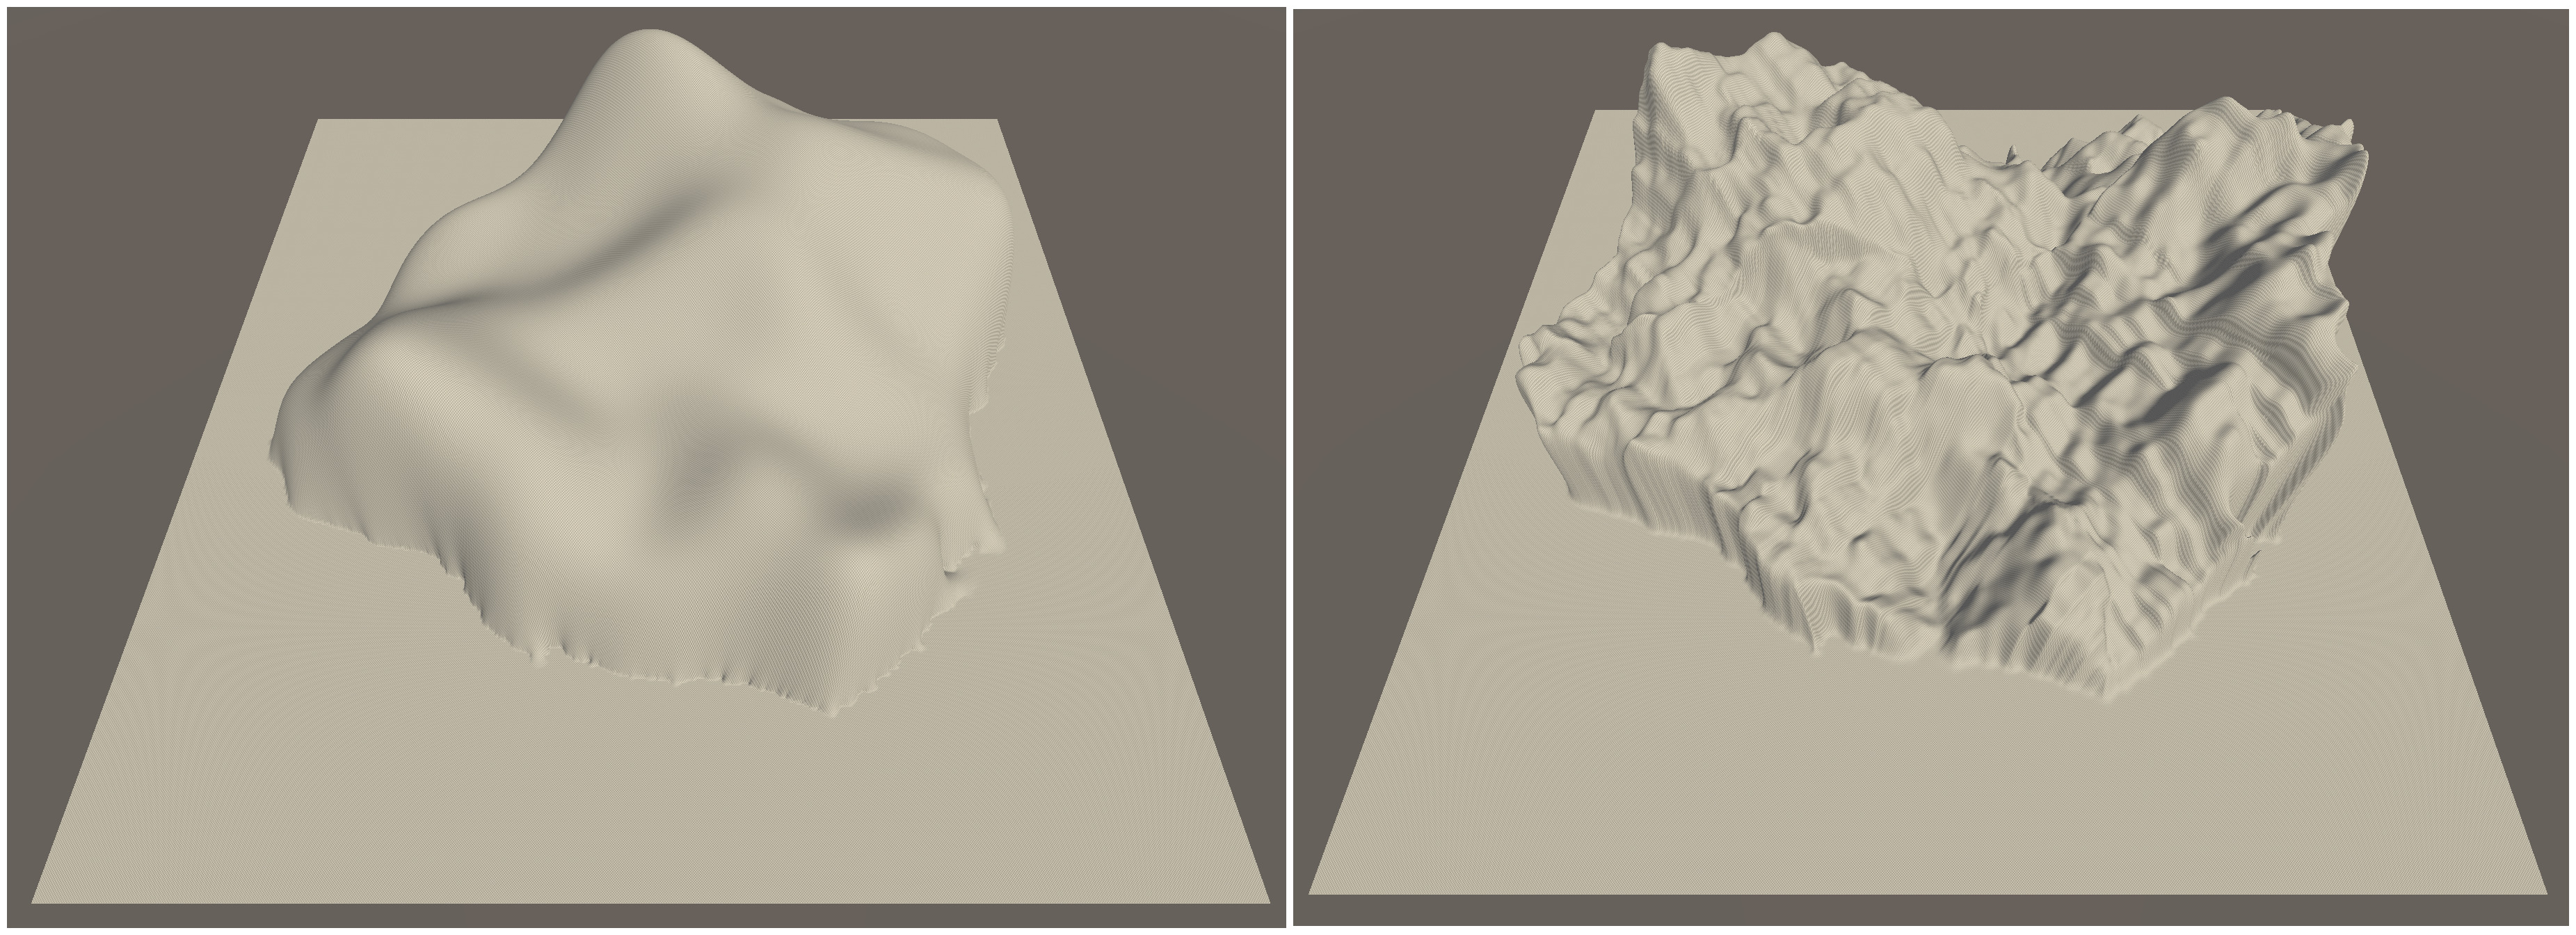
\includegraphics[width=1.0\textwidth]{img/distance_based_images/smoothing_comparison.jpg}
    \caption{Comparison of smoothing approaches on an island mask: (left) uniform smoothing loses terrain detail globally; (right) our enhanced distance-based smoothing preserves detail while creating more gentle transitions.}
    \label{fig:smoothing_comparison}
\end{figure}

\section{Distance-Based Height Scaling}
\label{dbhs}

While smoothing addresses local transitions by blending neighbouring heights, significant elevation disparities between fixed and generated areas require a fundamentally different approach. Our \textbf{distance-based height scaling} technique operates globally, adjusting the overall elevation profile of the terrain. Unlike smoothing, which preserves relative height differences while creating gradual transitions, height scaling actively modifies elevations to reduce the disparity between procedurally generated terrain and fixed constraints. 

This technique gradually adjusts terrain elevations by blending between the original procedural heights and a \textbf{reference height} -- a target elevation calculated from the fixed points' heights. The result is a terrain that naturally ``flows'' toward the constrained areas, creating realistic slopes and preventing the cliff-like formations that would otherwise appear at boundaries. The strength of how much it blends the original height towards the reference height is based on the distance to the nearest fixed point. This means that areas nearer to constraints will be closer in height to the reference height, and areas further away will maintain more of their procedurally generated height. 

Before explaining the relevant information and formal, mathematical formulation of distance-based height scaling, we present Figure \ref{fig:dbhs_effect} below to show the effects of this technique:

\begin{figure}[h!]
    \centering
    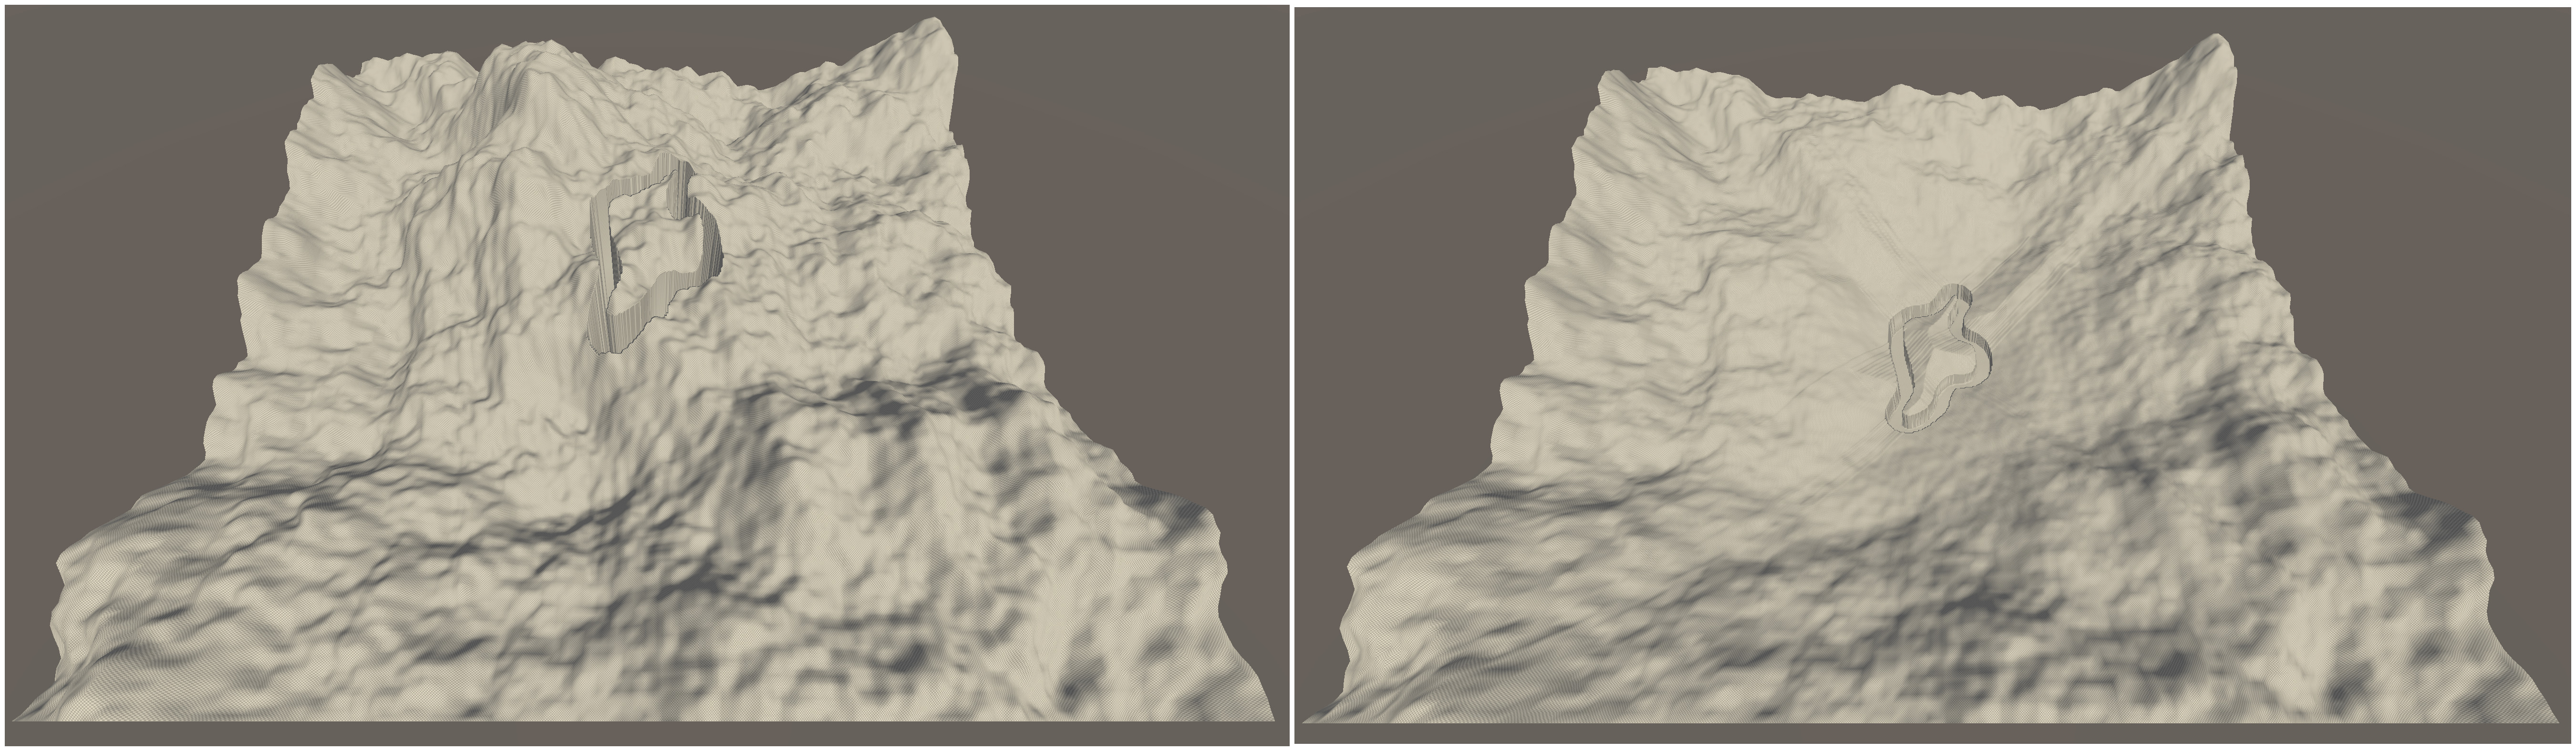
\includegraphics[width=1.0\textwidth]{img/distance_based_images/dbhs_effect.jpg}
    \caption{Distance-based height scaling effect: (Left) Perlin noise applied without any modifications to blend into the constraint, where the constraint in the middle of the terrain has abrupt transition to the surrounding area. (Right) After height scaling, showing reduced elevation disparities constraint and how the terrain now flows towards the heights of the constrained areas.}
    \label{fig:dbhs_effect}
\end{figure}

\subsubsection{Reference Height Selection}
\label{ref_height_selection}

The effectiveness of height scaling depends critically on choosing an appropriate reference height, as this is the target elevation toward which the terrain transitions. We calculate this reference height from the existing fixed points using one of three methods:

\begin{itemize}
    \item \textbf{Average Height} (default): Calculates the mean elevation of all fixed points, creating balanced transitions that work well for most constraints.
    
    \item \textbf{Minimum Height}: Uses the lowest elevation among fixed points, causing surrounding terrain to descend toward this level. 
    
    \item \textbf{Maximum Height}: Uses the highest elevation among fixed points, elevating surrounding terrain to create plateaus or mountain ranges around constrained peaks.
\end{itemize}

The choice of reference height method is not about correctness but about achieving the desired terrain characteristics. As demonstrated in Figures~\ref{fig:dbhs_base} and \ref{fig:dbhs_reference_heights}, each method produces distinctly different but \textit{equally} \textit{valid} terrain formations. The flexibility to choose between these methods allows artists and designers to achieve their specific vision while maintaining natural transitions.

\subsubsection{Mathematical Formulation}
Now we propose the mathematical approaches to this technique. The algorithm blends between original procedural heights, set by a traditional procedural terrain generation algorithm, and a reference height derived from fixed area heights. This can be formally represented as:

\[ h'(x, y) = h(x, y) \cdot s(d) + h_{ref} \cdot (1 - s(d)) \]

This equation performs a distance-weighted calculation where:

\begin{itemize}
    \item $h'(x,y)$ is the final scaled height at position $(x,y)$;
    \item $h(x,y)$ is the original procedural height at that position;
    \item  $h_{ref}$ is the \textbf{reference height} calculated from fixed points;
    \item $s(d)$ is the distance-based \textbf{scaling function} that controls the blend between original and reference heights:
    
    \[ s(d) = s_{min} + (1 - s_{min}) \cdot d_{norm} \]
\end{itemize}


The scaling function $s(d)$ creates a smooth transition, with $s_{norm}$ being the same as described in Section \ref{edbs_math}:
\begin{itemize}
    \item At fixed boundaries ($d_{norm} = 0$): $s(0) = s_{min}$, giving maximum influence to the reference height;
    \item At maximum distance ($d_{norm} = 1$): $s(1) = 1$, preserving the original procedural height
    \item $s_{min} \in [0, 1]$ controls the strength of the effect:
        \begin{itemize}
            \item $s_{min} = 0$: Complete flattening to reference height at boundaries;
            \item $s_{min} = 0.5$: 50\% blend between original and reference at boundaries;
            \item $s_{min} = 1$: No effect (original heights preserved everywhere).
        \end{itemize}
\end{itemize}

The final height calculation can be rewritten to show the blending more clearly:

\begin{equation}
h'(x, y) = \underbrace{h(x, y) \cdot s(d)}_{\text{scaled original}} + 
           \underbrace{h_{ref} \cdot (1 - s(d))}_{\text{reference contribution}}
\end{equation}

This mechanism can be rewritten as the following pseudocode:

\begin{algorithm}[H]
\small
\caption{Distance-Based Height Scaling}
\label{alg:height_scaling}
\begin{algorithmic}[1]
\Require $\text{heightMap}[w \times h]$, $\text{distanceGrid}[w \times h]$, $\text{params}$
\Ensure Height-scaled terrain with natural transitions to fixed areas

\State $h_{\text{ref}} \gets \text{calculateReference}(\text{heightMap}, \text{params.method})$
\State $\text{maxDistance} \gets \max(\text{distanceGrid})$

\For{each modifiable point $(x,y)$}
    \State $d_{\text{norm}} \gets \text{distanceGrid}[x,y] / \text{maxDistance}$
    
    \Comment{Scale factor increases with distance from fixed points}
    \State $s \gets \text{params.minScale} + (1 - \text{params.minScale}) \times d_{\text{norm}}$
    
    \Comment{Apply scaling to original height}
    \State $h_{\text{scaled}} \gets \text{heightMap}[x,y] \times s$
    
    \Comment{Calculate blend factor for reference height influence}
    \State $\text{blendFactor} \gets (1 - d_{\text{norm}}) \times (1 - s)$
    
    \Comment{Interpolate between scaled height and reference height}
    \State $\text{heightMap}[x,y] \gets \text{lerp}(h_{\text{scaled}}, h_{\text{ref}}, \text{blendFactor})$
\EndFor

\Function{lerp}{$a, b, t$}
    \State \Return $a \times (1 - t) + b \times t$
\EndFunction
\end{algorithmic}
\end{algorithm}

\textbf{Complexity Analysis}: The algorithm achieves excellent efficiency with $O(n)$ time complexity, processing each pixel exactly once. The reference height calculation adds an initial $O(n)$ scan of fixed points, and finding the maximum distance requires another $O(n)$ pass, but these are one-time costs. 

Figure~\ref{fig:dbhs_base} and \ref{fig:dbhs_reference_heights} demonstrate the visual impact of height scaling and how the different reference methods affect this.

\begin{figure}[h!]
    \centering
    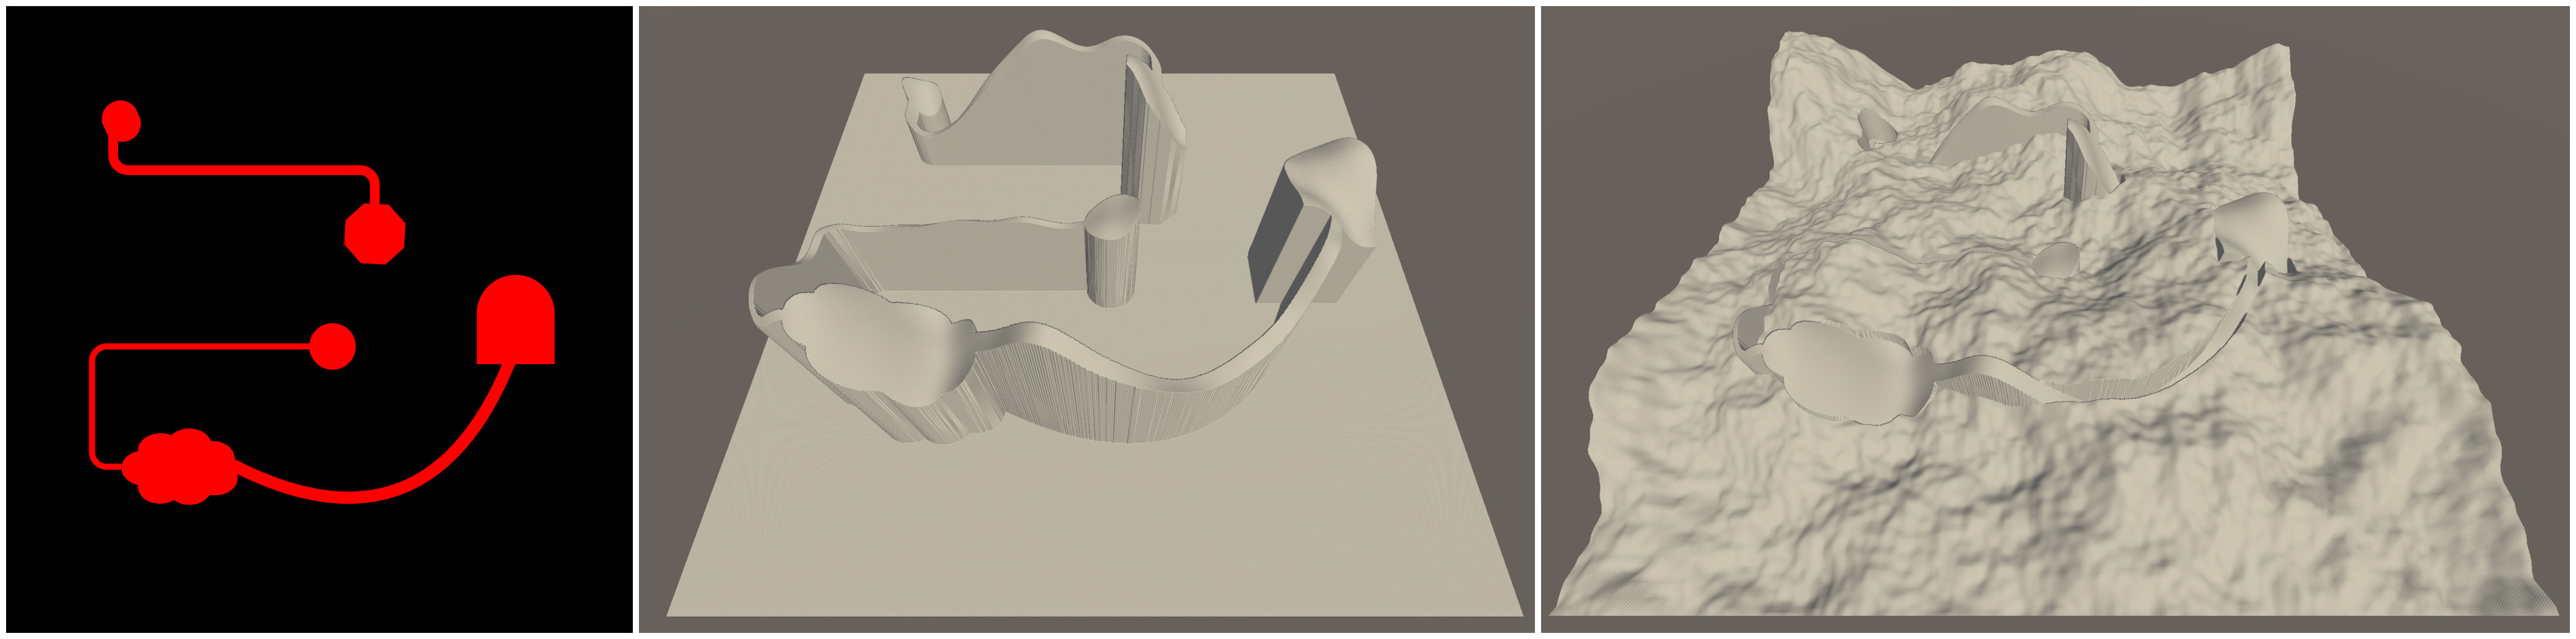
\includegraphics[width=1.0\textwidth]{img/distance_based_images/dbhs_base.jpg}
    \caption{Test terrain for demonstrating reference height methods: (Left) mask texture. (Middle) base terrain heights set in constrained areas. (Right) Perlin noise applied with no post-processing.}
    \label{fig:dbhs_base}
\end{figure}

\begin{figure}[h!]
    \centering
    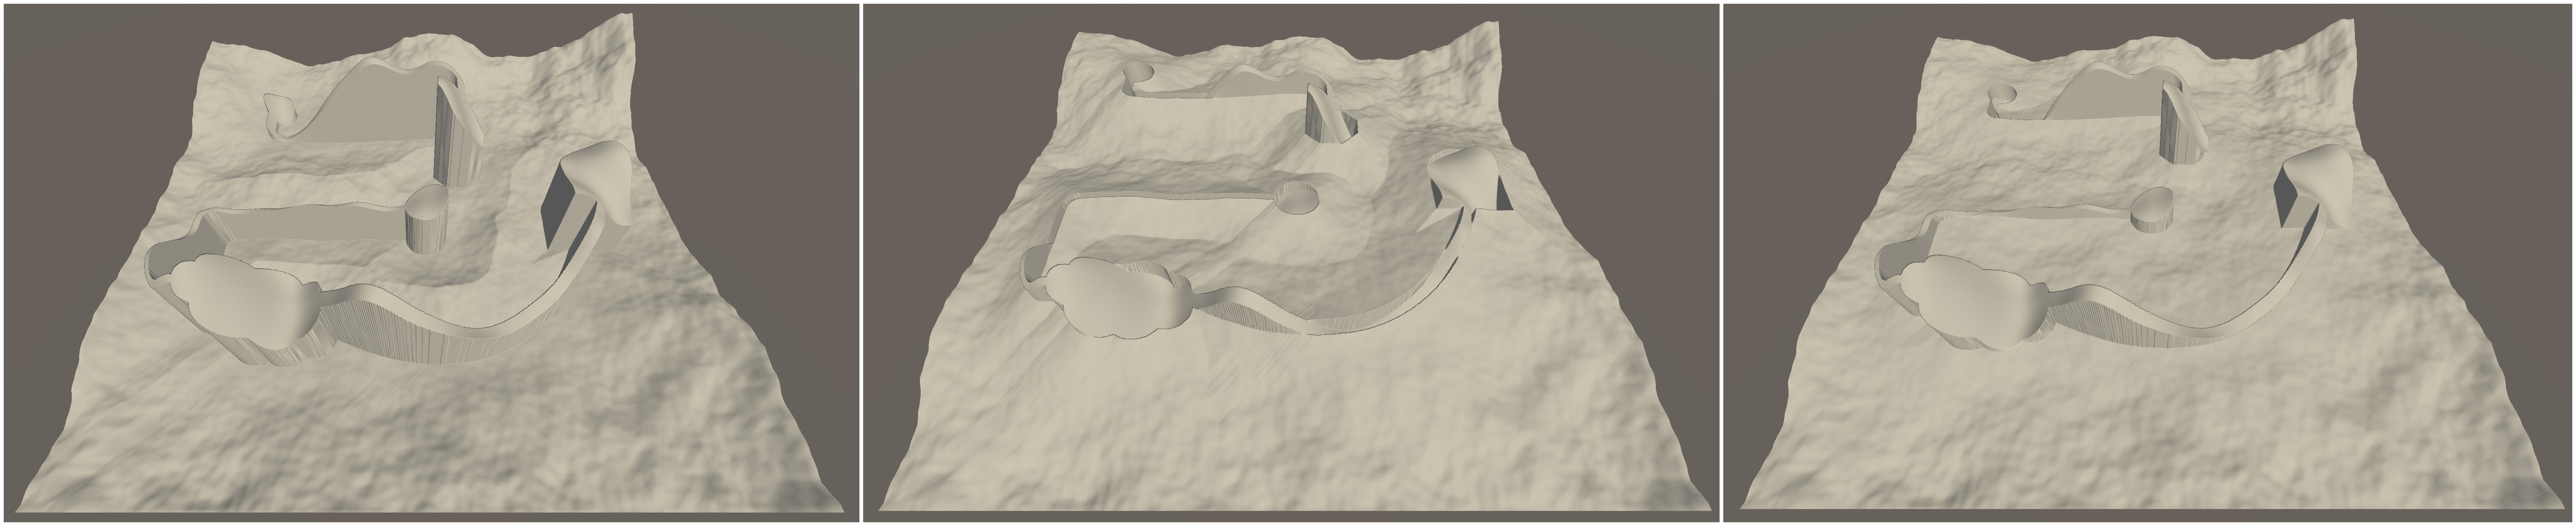
\includegraphics[width=1.0\textwidth]{img/distance_based_images/dbhs_reference_height.jpg}
    \caption{Effect of different reference heights when applying distance-based height scaling, applied to the example seen in Fig. \ref{fig:dbhs_base}. (Left) Minimum reference height used, creates valleys towards the minimum height of the constrained area. (Middle) Maximum reference height forms elevated regions around the constrained areas. (Right) Average of all constrained points as a reference height produces balanced transitions towards the mean height of the pixels in the constrained areas.}
    \label{fig:dbhs_reference_heights}
\end{figure}

\section{Summary}

This chapter presented our novel distance-based approach for creating natural transitions in constrained procedural terrain generation. By using distance from fixed points as a unifying metric, we achieve:

\begin{itemize}
    \item \textbf{Seamless integration}: Natural transitions that eliminate the boundary problem;
    \item \textbf{Algorithm independence}: Compatibility with any terrain generation technique;
    \item \textbf{Computational efficiency}: Linear $O(n)$ complexity for core operations with optional iteration-based smoothing;
    \item \textbf{Intuitive control}: Parameters with clear visual meaning.
\end{itemize}

The combination of distance-based height scaling and enhanced smoothing provides a complete solution, where height scaling addresses large-scale elevation disparities while distance-based smoothing refines local transitions without removing detail in distant areas. This two-stage approach produces terrain that appears naturally formed around fixed elements rather than artificially constrained.

Crucially, the computational efficiency of our algorithms, with single-pass $O(n)$ operations and GPU acceleration, enables the real-time feedback necessary for the Interactive Genetic Algorithm presented in Chapter~\ref{Chapter4}. Without this efficiency, the iterative parameter exploration that makes our system accessible to non-experts would be impractical. 